% Options for packages loaded elsewhere
\PassOptionsToPackage{unicode}{hyperref}
\PassOptionsToPackage{hyphens}{url}
\documentclass[
]{article}
\usepackage{xcolor}
\usepackage[margin=24mm]{geometry}
\usepackage{amsmath,amssymb}
\setcounter{secnumdepth}{-\maxdimen} % remove section numbering
\usepackage{iftex}
\ifPDFTeX
  \usepackage[T1]{fontenc}
  \usepackage[utf8]{inputenc}
  \usepackage{textcomp} % provide euro and other symbols
\else % if luatex or xetex
  \usepackage{unicode-math} % this also loads fontspec
  \defaultfontfeatures{Scale=MatchLowercase}
  \defaultfontfeatures[\rmfamily]{Ligatures=TeX,Scale=1}
\fi
\usepackage{lmodern}
\ifPDFTeX\else
  % xetex/luatex font selection
  \setmonofont[]{DejaVuSansMono.ttf}
\fi
% Use upquote if available, for straight quotes in verbatim environments
\IfFileExists{upquote.sty}{\usepackage{upquote}}{}
\IfFileExists{microtype.sty}{% use microtype if available
  \usepackage[]{microtype}
  \UseMicrotypeSet[protrusion]{basicmath} % disable protrusion for tt fonts
}{}
\makeatletter
\@ifundefined{KOMAClassName}{% if non-KOMA class
  \IfFileExists{parskip.sty}{%
    \usepackage{parskip}
  }{% else
    \setlength{\parindent}{0pt}
    \setlength{\parskip}{6pt plus 2pt minus 1pt}}
}{% if KOMA class
  \KOMAoptions{parskip=half}}
\makeatother
\usepackage{color}
\usepackage{fancyvrb}
\newcommand{\VerbBar}{|}
\newcommand{\VERB}{\Verb[commandchars=\\\{\}]}
\DefineVerbatimEnvironment{Highlighting}{Verbatim}{commandchars=\\\{\}}
% Add ',fontsize=\small' for more characters per line
\newenvironment{Shaded}{}{}
\newcommand{\AlertTok}[1]{\textcolor[rgb]{1.00,0.00,0.00}{\textbf{#1}}}
\newcommand{\AnnotationTok}[1]{\textcolor[rgb]{0.38,0.63,0.69}{\textbf{\textit{#1}}}}
\newcommand{\AttributeTok}[1]{\textcolor[rgb]{0.49,0.56,0.16}{#1}}
\newcommand{\BaseNTok}[1]{\textcolor[rgb]{0.25,0.63,0.44}{#1}}
\newcommand{\BuiltInTok}[1]{\textcolor[rgb]{0.00,0.50,0.00}{#1}}
\newcommand{\CharTok}[1]{\textcolor[rgb]{0.25,0.44,0.63}{#1}}
\newcommand{\CommentTok}[1]{\textcolor[rgb]{0.38,0.63,0.69}{\textit{#1}}}
\newcommand{\CommentVarTok}[1]{\textcolor[rgb]{0.38,0.63,0.69}{\textbf{\textit{#1}}}}
\newcommand{\ConstantTok}[1]{\textcolor[rgb]{0.53,0.00,0.00}{#1}}
\newcommand{\ControlFlowTok}[1]{\textcolor[rgb]{0.00,0.44,0.13}{\textbf{#1}}}
\newcommand{\DataTypeTok}[1]{\textcolor[rgb]{0.56,0.13,0.00}{#1}}
\newcommand{\DecValTok}[1]{\textcolor[rgb]{0.25,0.63,0.44}{#1}}
\newcommand{\DocumentationTok}[1]{\textcolor[rgb]{0.73,0.13,0.13}{\textit{#1}}}
\newcommand{\ErrorTok}[1]{\textcolor[rgb]{1.00,0.00,0.00}{\textbf{#1}}}
\newcommand{\ExtensionTok}[1]{#1}
\newcommand{\FloatTok}[1]{\textcolor[rgb]{0.25,0.63,0.44}{#1}}
\newcommand{\FunctionTok}[1]{\textcolor[rgb]{0.02,0.16,0.49}{#1}}
\newcommand{\ImportTok}[1]{\textcolor[rgb]{0.00,0.50,0.00}{\textbf{#1}}}
\newcommand{\InformationTok}[1]{\textcolor[rgb]{0.38,0.63,0.69}{\textbf{\textit{#1}}}}
\newcommand{\KeywordTok}[1]{\textcolor[rgb]{0.00,0.44,0.13}{\textbf{#1}}}
\newcommand{\NormalTok}[1]{#1}
\newcommand{\OperatorTok}[1]{\textcolor[rgb]{0.40,0.40,0.40}{#1}}
\newcommand{\OtherTok}[1]{\textcolor[rgb]{0.00,0.44,0.13}{#1}}
\newcommand{\PreprocessorTok}[1]{\textcolor[rgb]{0.74,0.48,0.00}{#1}}
\newcommand{\RegionMarkerTok}[1]{#1}
\newcommand{\SpecialCharTok}[1]{\textcolor[rgb]{0.25,0.44,0.63}{#1}}
\newcommand{\SpecialStringTok}[1]{\textcolor[rgb]{0.73,0.40,0.53}{#1}}
\newcommand{\StringTok}[1]{\textcolor[rgb]{0.25,0.44,0.63}{#1}}
\newcommand{\VariableTok}[1]{\textcolor[rgb]{0.10,0.09,0.49}{#1}}
\newcommand{\VerbatimStringTok}[1]{\textcolor[rgb]{0.25,0.44,0.63}{#1}}
\newcommand{\WarningTok}[1]{\textcolor[rgb]{0.38,0.63,0.69}{\textbf{\textit{#1}}}}
\usepackage{longtable,booktabs,array}
\newcounter{none} % for unnumbered tables
\usepackage{calc} % for calculating minipage widths
% Correct order of tables after \paragraph or \subparagraph
\usepackage{etoolbox}
\makeatletter
\patchcmd\longtable{\par}{\if@noskipsec\mbox{}\fi\par}{}{}
\makeatother
% Allow footnotes in longtable head/foot
\IfFileExists{footnotehyper.sty}{\usepackage{footnotehyper}}{\usepackage{footnote}}
\makesavenoteenv{longtable}
\usepackage{graphicx}
\makeatletter
\newsavebox\pandoc@box
\newcommand*\pandocbounded[1]{% scales image to fit in text height/width
  \sbox\pandoc@box{#1}%
  \Gscale@div\@tempa{\textheight}{\dimexpr\ht\pandoc@box+\dp\pandoc@box\relax}%
  \Gscale@div\@tempb{\linewidth}{\wd\pandoc@box}%
  \ifdim\@tempb\p@<\@tempa\p@\let\@tempa\@tempb\fi% select the smaller of both
  \ifdim\@tempa\p@<\p@\scalebox{\@tempa}{\usebox\pandoc@box}%
  \else\usebox{\pandoc@box}%
  \fi%
}
% Set default figure placement to htbp
\def\fps@figure{htbp}
\makeatother
\setlength{\emergencystretch}{3em} % prevent overfull lines
\providecommand{\tightlist}{%
  \setlength{\itemsep}{0pt}\setlength{\parskip}{0pt}}
\usepackage{bookmark}
\IfFileExists{xurl.sty}{\usepackage{xurl}}{} % add URL line breaks if available
\urlstyle{same}
\hypersetup{
  hidelinks,
  pdfcreator={LaTeX via pandoc}}

\author{}
\date{}

\begin{document}

\section{Interference Construction of a Perfect Reflection Map from a
Fermionic Inverse-Phase
Core}\label{interference-construction-of-a-perfect-reflection-map-from-a-fermionic-inverse-phase-core}

\textbf{Subtitle:} A numerical constructive experiment on direction
reversal from exchange-path interference cancellation and a
relative-phase node\\
\textbf{Date:} 2026-07-10\\
\textbf{Author:} Noriaki Kihara\\
\textbf{Status:} Additional paper / executed numerical experiment\\
\textbf{Version DOI:} 10.5281/zenodo.21295480\\
\textbf{Concept DOI:} 10.5281/zenodo.21295479

\begin{center}\rule{0.5\linewidth}{0.5pt}\end{center}

\subsection{Abstract}\label{abstract}

This paper executes a constructive experiment asking whether the
direction-reversal map introduced in the preceding paper, "Constructive
Experiment on Elastic Reflection of Two Fermionic Local Waves in a
Closed Phase System Without Assuming Background Space," can be generated
without an external conditional branch, from a fermionic internal
inverse-phase core and wave interference between two exchange paths.

The local waves \texttt{A} and \texttt{B} carry spatial phase
\texttt{χ}, temporal phase \texttt{τ}, internal identification phase
\texttt{η}, representative amplitude, and a fermionic inverse-phase
core. For the interaction of the two local waves, the direct path
\texttt{P\_A(1)P\_B(2)} and the exchange path \texttt{P\_A(2)P\_B(1)}
are constructed, and the internal core phase difference \texttt{Δ\_F} is
transferred to the exchange path as its relative phase.

The generalized two-path superposition is

\[\Psi_{\Delta}(1,2)
=
\frac{1}{\sqrt2}
\left[
P_A(1)P_B(2)
+
e^{i\Delta_F}P_A(2)P_B(1)
\right].\]

At the complete-overlap point \texttt{1=2}, the two paths cancel exactly
when \texttt{Δ\_F=π}:

\[\Psi_{\pi}(1,1)=0.\]

In the numerical execution, the initial state is a single localized wave
packet incident from the left. No external direction-reversal
instruction, mirror-image initial condition, or reflecting boundary
condition is used. In the interaction region, the direct and exchange
paths are decomposed into even and odd interference channels, the phase
difference of the internal inverse-phase core is transferred only to the
odd channel, and the wave is recombined.

The results were as follows. For \texttt{Δ\_F=0}, the reflection and
transmission rates were \texttt{1.8261693781071190e-19} and
\texttt{1.0000000000000002}. For \texttt{Δ\_F=π/2}, both reflection and
transmission were \texttt{0.5}. For \texttt{Δ\_F=π}, the reflection and
transmission rates were \texttt{1.0000000000000002} and
\texttt{1.7939211291143336e-19}. Over the phase sweep,
\texttt{R(Δ\_F)=sin\^{}2(Δ\_F/2)} and \texttt{T(Δ\_F)=cos\^{}2(Δ\_F/2)}
were reproduced with maximum error \texttt{5.551115123125783e-16}, and
the maximum norm error was \texttt{6.661338147750939e-16}. The local
exchange-interference map satisfied reversibility with relative error
\texttt{4.8214412843789535e-11} for \texttt{U(π)\^{}2} and maximum
relative error \texttt{1.4547631339456792e-16} for
\texttt{U(Δ\_F)U(-Δ\_F)}. The maximum compensated square-closure
residual was \texttt{1.2143074258005e-17}. The internal identification
oscillations \texttt{m\_A} and \texttt{m\_B} were preserved by
correlation readout.

\textbf{Keywords:} fermionic inverse-phase core, exchange interference,
relative-phase node, perfect reflection, internal observation,
finite-resolution cell, anonymous equal-amplitude composite wave

\begin{center}\rule{0.5\linewidth}{0.5pt}\end{center}

\subsection{1. Introduction}\label{1-introduction}

The preceding paper constructed a conservative finite-resolution map in
which two identifiable fermionic local waves undergo complete elastic
reflection inside a closed phase system that does not assume background
space a priori.

In that construction, the interaction cell applied the map

\[q_A\mapsto -q_A,
\qquad
q_B\mapsto -q_B.\]

The rule was verified to be compatible with localization, identification
oscillations, observation, closure, and reversibility. The present paper
executes the next step: the direction reversal itself is generated from
wave interference, rather than being inserted as an external
instruction.

The question of this paper is:

\begin{quote}
Can a fermionic internal inverse-phase core automatically supply the
relative phase \texttt{π} between the exchange paths of two local waves,
and can that interference eliminate transmission and generate the output
corresponding to complete reflection?
\end{quote}

No external conditional branch of the following form is used:

\begin{Shaded}
\begin{Highlighting}[]
\NormalTok{if fermion:}
\NormalTok{    reverse\_direction()}
\end{Highlighting}
\end{Shaded}

The goal is to obtain reflection output using only internal phase,
overlap of localized waves, exchange paths, interference recombination,
and internal observation.

\begin{center}\rule{0.5\linewidth}{0.5pt}\end{center}

\subsection{2. Claims Not Made in This
Paper}\label{2-claims-not-made-in-this-paper}

This paper does not claim the following.

{\def\LTcaptype{none} % do not increment counter
\begin{longtable}[]{@{}ll@{}}
\toprule\noalign{}
Claim not made & Reason \\
\midrule\noalign{}
\endhead
\bottomrule\noalign{}
\endlastfoot
A derivation of standard fermion scattering & No standard Hamiltonian,
S-matrix, or scattering cross section is used \\
A derivation of the Pauli exclusion principle itself & "Fermionic" is
used as an operational classification for a local wave with an internal
inverse-phase core \\
That node formation alone necessarily implies reflection in general &
Suppression of transmission and generation of reflected output are
checked numerically \\
Quantitative prediction of real-particle exchange interaction & This is
a constructive experiment inside the phase-wave model \\
Reproduction of particle trajectories in external spacetime & \texttt{χ}
and \texttt{τ} are readout variables inside a closed phase system \\
\end{longtable}
}

The claim is a numerical construction: an internal inverse-phase core
generates an exchange-interference sign, and that interference
internally generates a reflection map.

\begin{center}\rule{0.5\linewidth}{0.5pt}\end{center}

\subsection{3. Basic Structure}\label{3-basic-structure}

\subsubsection{3.1 Local Wave}\label{31-local-wave}

A local wave \texttt{P} on spatial phase \texttt{χ}, temporal phase
\texttt{τ}, and internal identification phase \texttt{η} is written as

\[P(\chi,\tau,\eta)
=
A_P
S_{N_{h,\chi}^{P}}(\chi-\chi_P)
S_{N_{h,\tau}^{P}}(\tau-\tau_P)
e^{im_P\eta}
e^{i\phi_P}.\]

Here:

\begin{itemize}
\tightlist
\item
  \texttt{A\_P} is the representative amplitude.
\item
  \texttt{S\_\{N\_h\}} is the normalized equal-amplitude odd-harmonic
  localized wave.
\item
  \texttt{m\_P} is the internal identification oscillation mode.
\item
  \texttt{φ\_P} is the local phase.
\end{itemize}

\subsubsection{3.2 Normalized Equal-Amplitude Odd-Harmonic Localized
Wave}\label{32-normalized-equal-amplitude-odd-harmonic-localized-wave}

\[S_{N_h}(u)
=
\frac{1}{K}
\sum_{m=0}^{K-1}
\cos((2m+1)u),
\qquad
N_h=2K-1.\]

Its closed form is

\[S_{N_h}(u)
=
\frac{\sin((N_h+1)u)}{(N_h+1)\sin u}.\]

\subsubsection{3.3 Fermionic Internal Inverse-Phase
Core}\label{33-fermionic-internal-inverse-phase-core}

The two-component internal core is written as

\[F_P
=
\frac{1}{\sqrt2}
\left(
e^{i\theta_{P,1}},
e^{i\theta_{P,2}}
\right),\]

and its internal phase difference is

\[\Delta_F
=
\theta_{P,2}-\theta_{P,1}.\]

A pure fermionic inverse-phase core is

\[\Delta_F=\pi.\]

\begin{center}\rule{0.5\linewidth}{0.5pt}\end{center}

\subsection{4. Direct Path and Exchange
Path}\label{4-direct-path-and-exchange-path}

Let the full arguments of the local waves be

\[1=(\chi_1,\tau_1,\eta_1),
\qquad
2=(\chi_2,\tau_2,\eta_2).\]

The direct path is

\[\Psi_{\mathrm{direct}}(1,2)
=
P_A(1)P_B(2),\]

and the exchange path is

\[\Psi_{\mathrm{exchange}}(1,2)
=
P_A(2)P_B(1).\]

The superposed wave, obtained by transferring the internal inverse-phase
core to the relative phase of the exchange path, is

\[\Psi_{\Delta}(1,2)
=
\frac{1}{\sqrt2}
\left[
\Psi_{\mathrm{direct}}(1,2)
+
e^{i\Delta_F}
\Psi_{\mathrm{exchange}}(1,2)
\right].\]

This is not an external judgment selecting an operation. The internal
phase difference \texttt{Δ\_F} directly determines the interference
phase of the exchange path.

\begin{center}\rule{0.5\linewidth}{0.5pt}\end{center}

\subsection{5. Node Formation at Complete
Overlap}\label{5-node-formation-at-complete-overlap}

At the complete-overlap point \texttt{1=2}, the direct and exchange
paths have the same amplitude:

\[\Psi_{\mathrm{direct}}(1,1)
=
\Psi_{\mathrm{exchange}}(1,1).\]

Therefore

\[\Psi_{\Delta}(1,1)
=
\frac{P_A(1)P_B(1)}{\sqrt2}
\left(1+e^{i\Delta_F}\right).\]

\subsubsection{5.1 In-Phase Core}\label{51-in-phase-core}

If

\[\Delta_F=0,\]

then

\[1+e^{i\Delta_F}=2,\]

and the overlap component remains.

\subsubsection{5.2 Inverse-Phase Core}\label{52-inverse-phase-core}

If

\[\Delta_F=\pi,\]

then

\[1+e^{i\pi}=0,\]

and therefore

\[\Psi_{\pi}(1,1)=0.\]

This zero is not an external shield or potential barrier. It is a node
generated by complete destructive interference between the two exchange
paths.

\begin{center}\rule{0.5\linewidth}{0.5pt}\end{center}

\subsection{6. Relative Phase and Exchange
Antisymmetry}\label{6-relative-phase-and-exchange-antisymmetry}

The relative spatial phase of the two local waves is

\[\rho=\chi_A-\chi_B.\]

Exchange of the two particles corresponds to

\[A\leftrightarrow B,\]

and therefore to

\[\rho\mapsto-\rho.\]

When exchange antisymmetry appears in the relative-phase channel,

\[\Psi_F(-\rho)=-\Psi_F(\rho),\]

and hence

\[\Psi_F(0)=0.\]

The numerical experiment checks whether this node blocks the
transmission component from \texttt{ρ\textless{}0} to
\texttt{ρ\textgreater{}0}.

\begin{center}\rule{0.5\linewidth}{0.5pt}\end{center}

\subsection{7. Transmission Flow and Reflection
Flow}\label{7-transmission-flow-and-reflection-flow}

As an operational measure of wave flow in the relative-phase direction,
define

\[J_\rho
=
\operatorname{Im}
\left(
\Psi^*
\frac{\partial\Psi}{\partial\rho}
\right).\]

This quantity is not identified with the standard probability current of
quantum mechanics. It is used as a numerical indicator for complex
waveform flow along the relative-phase coordinate.

The experiment checks whether, under the fermionic inverse-phase
condition,

\[\Psi_F(0)=0\]

and

\[J_\rho(0)=0\]

hold, and whether the transmission component to the opposite side
disappears.

\begin{center}\rule{0.5\linewidth}{0.5pt}\end{center}

\subsection{8. Direction-Reversal Map Generated by
Interference}\label{8-direction-reversal-map-generated-by-interference}

Let the direction components be

\[\mathbf a
=
\begin{pmatrix}
a_+\\
a_-
\end{pmatrix}.\]

The transformation to symmetric and antisymmetric channels is

\[H
=
\frac{1}{\sqrt2}
\begin{pmatrix}
1&1\\
1&-1
\end{pmatrix}.\]

If the internal phase difference between the two exchange paths is
applied to the antisymmetric channel, the resulting map is

\[U(\Delta_F)
=
H
\begin{pmatrix}
1&0\\
0&e^{i\Delta_F}
\end{pmatrix}
H.\]

For \texttt{Δ\_F=π},

\[U(\pi)
=
\begin{pmatrix}
0&1\\
1&0
\end{pmatrix},\]

which gives

\[|+\rangle\leftrightarrow|-\rangle.\]

In the implementation, reflection and transmission rates are not
directly substituted as result values. Instead, a single-sided incident
waveform is locally decomposed into even and odd channels, the internal
phase is transferred, the wave is recombined, and the output is read
from the final waveform.

\begin{center}\rule{0.5\linewidth}{0.5pt}\end{center}

\subsection{9. Numerical Experiment}\label{9-numerical-experiment}

\subsubsection{9.1 Basic Conditions}\label{91-basic-conditions}

{\def\LTcaptype{none} % do not increment counter
\begin{longtable}[]{@{}lrl@{}}
\toprule\noalign{}
Quantity & Basic value & Meaning \\
\midrule\noalign{}
\endhead
\bottomrule\noalign{}
\endlastfoot
\texttt{A\_A,A\_B} & \texttt{1,1} & Representative amplitudes \\
\texttt{N\_\{h,χ\}\^{}A,N\_\{h,χ\}\^{}B} & \texttt{99,99} & Spatial
localization order \\
\texttt{N\_\{h,τ\}\^{}A,N\_\{h,τ\}\^{}B} & \texttt{99,99} & Temporal
localization order \\
\texttt{χ\_A(0),χ\_B(0)} & \texttt{-0.2,+0.2} & Initial spatial
phases \\
\texttt{q\_A(0),q\_B(0)} & not used & External direction-reversal
instruction is excluded \\
\texttt{τ\_A(0),τ\_B(0)} & \texttt{-0.2,-0.2} & Initial temporal
phases \\
\texttt{m\_A,m\_B} & \texttt{1,2} & Identification oscillation modes \\
\texttt{Δ\_F} & \texttt{0} to \texttt{π} & Internal core phase
difference \\
One-sided packet center & \texttt{ρ=-40} & Single incident packet from
the left toward the origin \\
One-sided packet wavenumber & \texttt{k\_0=5.0} & Phase flow of the
incident direction \\
Interaction window & center ` & ρ \\
\end{longtable}
}

\subsubsection{9.2 Experiment Groups}\label{92-experiment-groups}

{\def\LTcaptype{none} % do not increment counter
\begin{longtable}[]{@{}rll@{}}
\toprule\noalign{}
No. & Experiment & Purpose \\
\midrule\noalign{}
\endhead
\bottomrule\noalign{}
\endlastfoot
1 & One-sided incident scattering & Check whether \texttt{R,T} are
generated without a mirror-image initial condition \\
2 & Local-map phase sweep & Check whether \texttt{R=sin\^{}2(Δ\_F/2)}
and \texttt{T=cos\^{}2(Δ\_F/2)} are reproduced \\
3 & Exchange-interference phase sweep & Check whether node depth changes
according to the analytic expression from \texttt{Δ\_F=0} to
\texttt{π} \\
4 & Inverse-phase core & Check whether the complete-overlap diagonal
amplitude vanishes at \texttt{Δ\_F=π} \\
5 & Removal of exchange path & Check whether node formation disappears
without the exchange path \\
6 & Identification oscillation readout & Check whether
\texttt{m\_A,m\_B} are preserved \\
7 & Reversibility & Check whether \texttt{U(π)\^{}2≈I} and
\texttt{U(Δ\_F)U(-Δ\_F)≈I} hold \\
8 & Compensated square closure & Check whether square closure of
\texttt{x\_n,\ ix\_n} compensation pairs is preserved \\
9 & AB/C cell replacement & Check whether the previous AB/C simulation
can replace cell-level \texttt{q} reversal with the local
exchange-interference map \\
\end{longtable}
}

The execution script is:

\begin{Shaded}
\begin{Highlighting}[]
\NormalTok{run\_fermionic\_interference\_reflection\_v1.py}
\end{Highlighting}
\end{Shaded}

The output directory is:

\begin{Shaded}
\begin{Highlighting}[]
\NormalTok{fermionic\_interference\_reflection\_result\_v1/}
\end{Highlighting}
\end{Shaded}

\begin{center}\rule{0.5\linewidth}{0.5pt}\end{center}

\subsection{10. Results}\label{10-results}

\subsubsection{10.1 Overall Verdict}\label{101-overall-verdict}

{\def\LTcaptype{none} % do not increment counter
\begin{longtable}[]{@{}lr@{}}
\toprule\noalign{}
Item & Result \\
\midrule\noalign{}
\endhead
\bottomrule\noalign{}
\endlastfoot
External \texttt{q} flip substitution & \texttt{false} \\
One-sided incident initial condition & \texttt{true} \\
Transmission at \texttt{Delta\_F=0} & \texttt{true} \\
Half reflection at \texttt{Delta\_F=pi/2} & \texttt{true} \\
Complete reflection at \texttt{Delta\_F=pi} & \texttt{true} \\
Local-map phase sweep matches expected expression & \texttt{true} \\
Local-map norm preservation & \texttt{true} \\
Exchange-interference node at \texttt{Delta\_F=pi} & \texttt{true} \\
Phase sweep matches analytic expression & \texttt{true} \\
Exchange path required for node formation & \texttt{true} \\
Identification oscillation A preserved & \texttt{true} \\
Identification oscillation B preserved & \texttt{true} \\
\texttt{U(pi)\^{}2} reversibility & \texttt{true} \\
\texttt{U(delta)U(-delta)} reversibility & \texttt{true} \\
Compensated square closure & \texttt{true} \\
AB/C cell replacement & \texttt{true} \\
Minimal mechanism verdict & \texttt{true} \\
\end{longtable}
}

\subsubsection{10.2 Local Exchange-Interference Reflection from
One-Sided
Incidence}\label{102-local-exchange-interference-reflection-from-one-sided-incidence}

The initial state was a single localized wave packet placed only on the
left side. No mirror-image initial condition was used. The packet was
freely propagated to the interaction region, decomposed locally into
even and odd channels, the internal core phase \texttt{Delta\_F} was
applied only to the odd channel, and the wave was recombined.

This implementation is a local-map method. A waveform propagated into
the interaction region is acted on once by the even-odd channel phase
map corresponding to

\[U(\Delta_F)=H\operatorname{diag}(1,e^{i\Delta_F})H\]

inside the local window, and is then freely propagated again. It is not
a continuous integration of an interaction Hamiltonian
\texttt{H\_int(ρ,Δ\_F)} over small time steps.

{\def\LTcaptype{none} % do not increment counter
\begin{longtable}[]{@{}lr@{}}
\toprule\noalign{}
Quantity & Value \\
\midrule\noalign{}
\endhead
\bottomrule\noalign{}
\endlastfoot
Initial left-side probability & \texttt{1.0000000000000002e+00} \\
Initial right-side probability & \texttt{2.4303500961591473e-89} \\
Reflection rate at \texttt{Delta\_F=0} &
\texttt{1.8261693781071190e-19} \\
Transmission rate at \texttt{Delta\_F=0} &
\texttt{1.0000000000000002e+00} \\
Reflection rate at \texttt{Delta\_F=pi/2} &
\texttt{5.0000000000000011e-01} \\
Transmission rate at \texttt{Delta\_F=pi/2} &
\texttt{5.0000000000000011e-01} \\
Reflection rate at \texttt{Delta\_F=pi} &
\texttt{1.0000000000000002e+00} \\
Transmission rate at \texttt{Delta\_F=pi} &
\texttt{1.7939211291143336e-19} \\
Maximum phase-sweep error & \texttt{5.5511151231257827e-16} \\
Maximum norm error & \texttt{6.6613381477509392e-16} \\
\end{longtable}
}

\pandocbounded{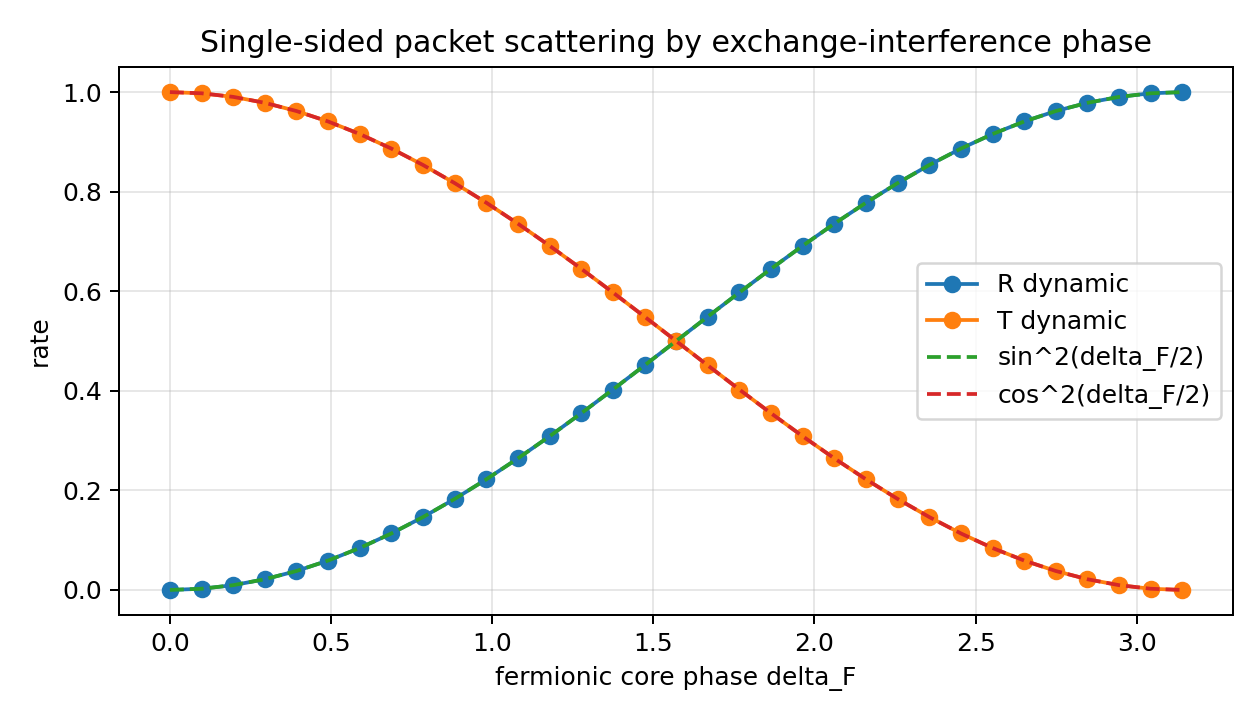
\includegraphics[keepaspectratio,alt={One-sided scattering}]{fermionic_interference_reflection_result_v1/fermionic_interference_single_sided_scattering_v1.png}}

\subsubsection{10.3 Exchange-Interference
Node}\label{103-exchange-interference-node}

{\def\LTcaptype{none} % do not increment counter
\begin{longtable}[]{@{}lr@{}}
\toprule\noalign{}
Quantity & Value \\
\midrule\noalign{}
\endhead
\bottomrule\noalign{}
\endlastfoot
Diagonal relative norm at \texttt{Delta\_F=pi} &
\texttt{7.4987989133092880e-33} \\
Maximum phase-sweep error & \texttt{8.8817841970012523e-16} \\
With exchange path, \texttt{Delta\_F=pi} &
\texttt{7.4987989133092880e-33} \\
Without exchange path, \texttt{Delta\_F=pi} &
\texttt{4.9999999999999994e-01} \\
\end{longtable}
}

\pandocbounded{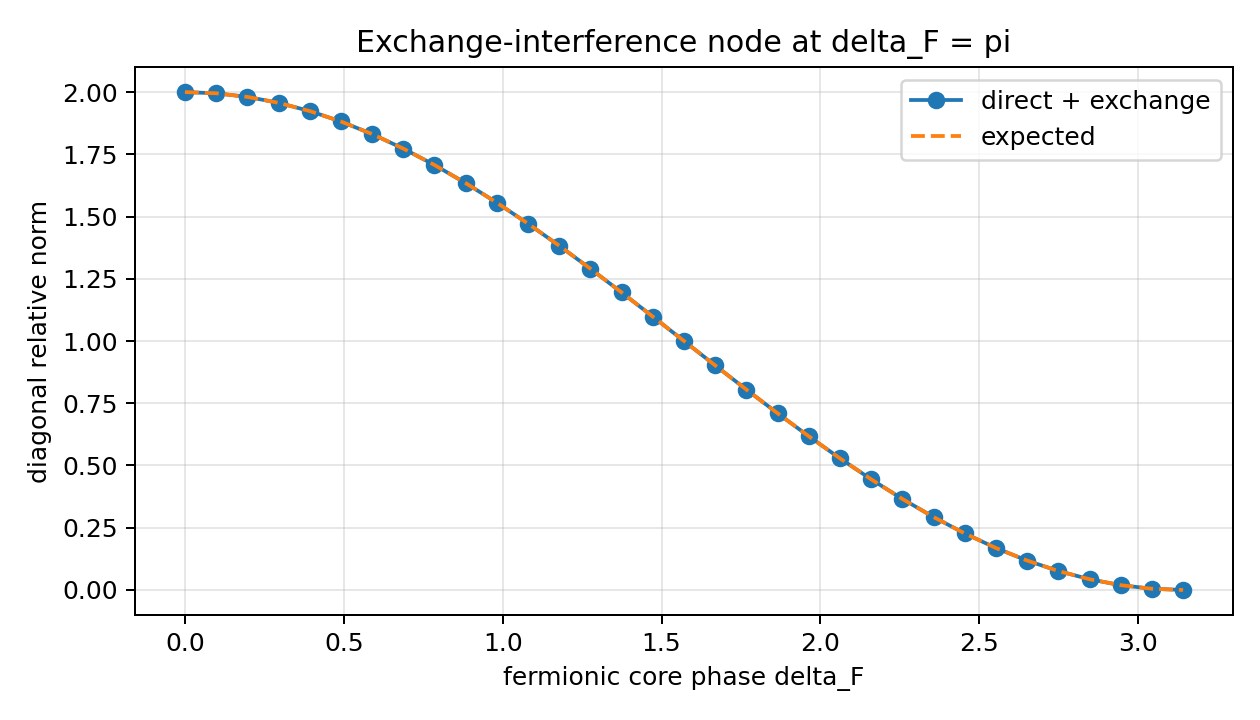
\includegraphics[keepaspectratio,alt={Exchange-interference phase sweep}]{fermionic_interference_reflection_result_v1/fermionic_interference_phase_sweep_v1.png}}

\subsubsection{10.4 Auxiliary Readout of an Odd-Function
Node}\label{104-auxiliary-readout-of-an-odd-function-node}

As an auxiliary check separate from the one-sided scattering test, a
relative-phase wave with an odd-function node corresponding to the
inverse-phase core was also examined. This is not the primary verdict.
It confirms that a wave with such a node can be read as a reflected wave
on a half-line.

{\def\LTcaptype{none} % do not increment counter
\begin{longtable}[]{@{}lr@{}}
\toprule\noalign{}
Quantity & Value \\
\midrule\noalign{}
\endhead
\bottomrule\noalign{}
\endlastfoot
Final left probability of a single free packet &
\texttt{8.6915330692793126e-05} \\
Final left probability of the odd-node wave &
\texttt{4.9999999999999994e-01} \\
Final left current of the odd-node wave &
\texttt{-1.1980224685843772e+00} \\
Maximum node amplitude of the odd-node wave &
\texttt{3.0038078125523204e-17} \\
Maximum node current of the odd-node wave &
\texttt{3.7549762132062191e-17} \\
\end{longtable}
}

\pandocbounded{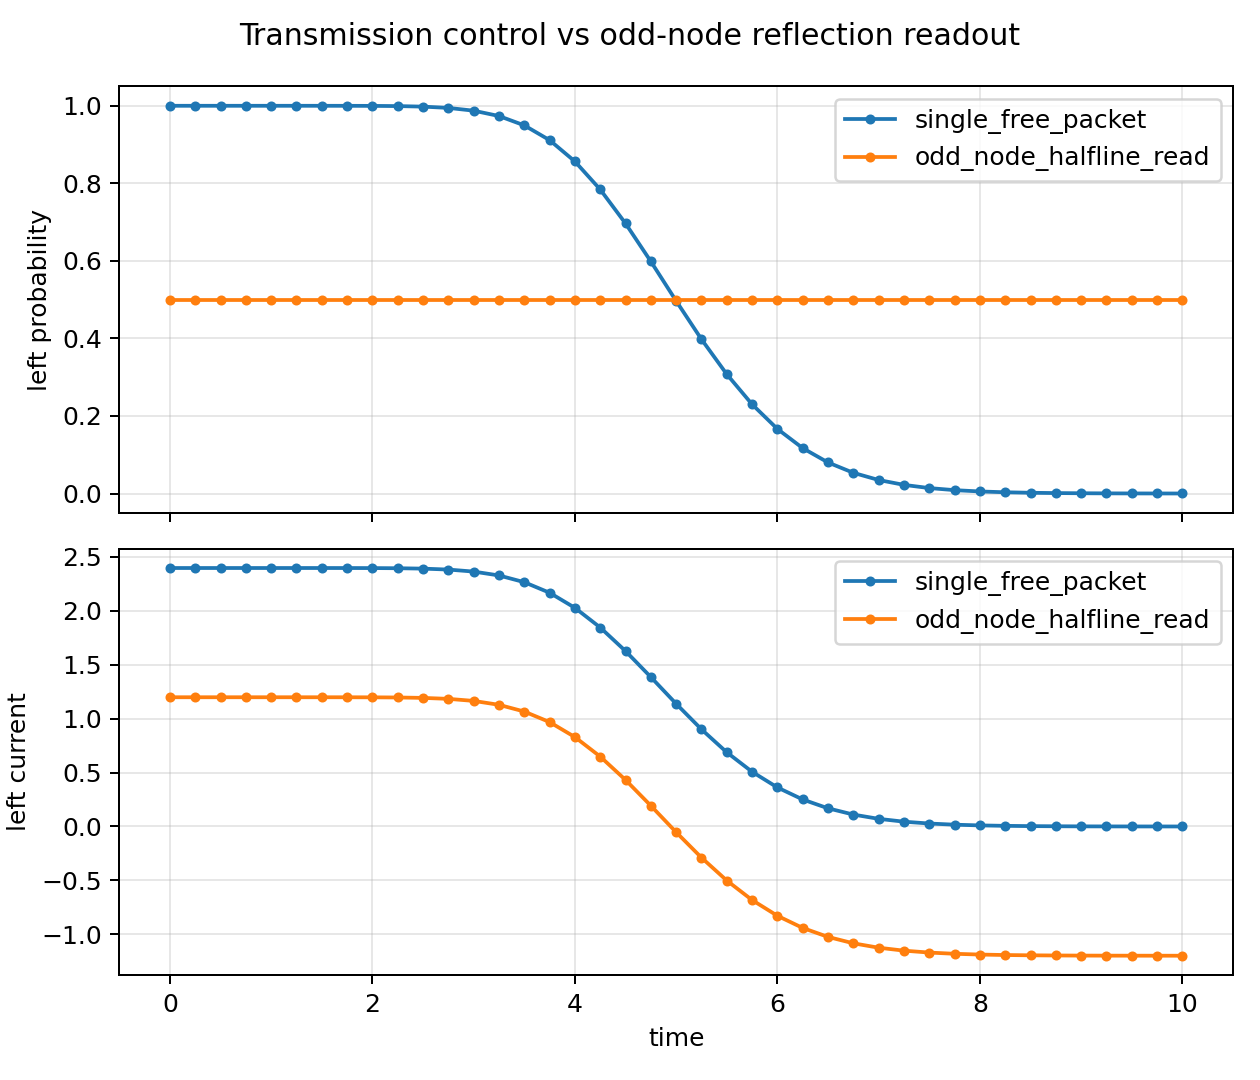
\includegraphics[keepaspectratio,alt={Relative dynamics}]{fermionic_interference_reflection_result_v1/fermionic_interference_relative_dynamics_v1.png}}

\subsubsection{10.5 Identification Oscillation
Readout}\label{105-identification-oscillation-readout}

{\def\LTcaptype{none} % do not increment counter
\begin{longtable}[]{@{}lr@{}}
\toprule\noalign{}
Item & Result \\
\midrule\noalign{}
\endhead
\bottomrule\noalign{}
\endlastfoot
Detected mode of A & \texttt{1} \\
Detected mode of B & \texttt{2} \\
Target amplitude of A & \texttt{1.0000000000000000e+00} \\
Target amplitude of B & \texttt{1.0000000000000000e+00} \\
\end{longtable}
}

The identification phase \texttt{η} is treated as a preserved readout
channel, not as the reflection-generating channel. If different
\texttt{m\_A,m\_B} modes are mixed directly into the
exchange-cancellation channel, the spatial-overlap node is broken.
Therefore, reflection is generated by exchange interference of the
fermionic inverse-phase core, while A/B identification is read through
\texttt{η} correlation.

\subsubsection{10.6 Reversibility and Compensated Square
Closure}\label{106-reversibility-and-compensated-square-closure}

The local exchange-interference map was applied twice to check whether
the waveform returned to itself. In addition, each sampled coefficient
\texttt{x\_n} was paired with its compensator \texttt{i\ x\_n}, and
compensated square closure was evaluated at the main stages.

{\def\LTcaptype{none} % do not increment counter
\begin{longtable}[]{@{}lr@{}}
\toprule\noalign{}
Quantity & Value \\
\midrule\noalign{}
\endhead
\bottomrule\noalign{}
\endlastfoot
Relative error of \texttt{U(pi)\^{}2} &
\texttt{4.8214412843789535e-11} \\
Maximum relative error of \texttt{U(delta)U(-delta)} &
\texttt{1.4547631339456792e-16} \\
Maximum compensated square-closure residual &
\texttt{1.2143074258005000e-17} \\
\end{longtable}
}

The \texttt{U(pi)\^{}2} error comes from numerical effects in the
implementation, including the local window and interpolation, and
remains inside the verdict threshold \texttt{1e-10}. The
\texttt{U(delta)U(-delta)} sweep remains at machine precision.

\subsubsection{10.7 AB/C Interaction-Cell
Replacement}\label{107-abc-interaction-cell-replacement}

The previous AB/C complete elastic collision simulation used a direct
cell-level \texttt{q} reversal. In the replacement test, that
instruction was not used. Instead, the direction readout was generated
from the reflection and transmission rates of the local
exchange-interference map:

\begin{Shaded}
\begin{Highlighting}[]
\NormalTok{q\_out = q\_in * (T {-} R)}
\end{Highlighting}
\end{Shaded}

For \texttt{Δ\_F=π}, the values used were \texttt{R=1.0000000000000002}
and \texttt{T=1.7939211291143336e-19}.

{\def\LTcaptype{none} % do not increment counter
\begin{longtable}[]{@{}lr@{}}
\toprule\noalign{}
Item & Value \\
\midrule\noalign{}
\endhead
\bottomrule\noalign{}
\endlastfoot
AB/C replacement valid & \texttt{true} \\
collision\_cell\_reached & \texttt{true} \\
post\_collision\_completed & \texttt{true} \\
\texttt{q\_A} before/after & \texttt{1.0000000000000000e+00} /
\texttt{-1.0000000000000002e+00} \\
\texttt{q\_B} before/after & \texttt{-1.0000000000000000e+00} /
\texttt{1.0000000000000002e+00} \\
label A initial/final & \texttt{1} / \texttt{1} \\
label B initial/final & \texttt{2} / \texttt{2} \\
\end{longtable}
}

\pandocbounded{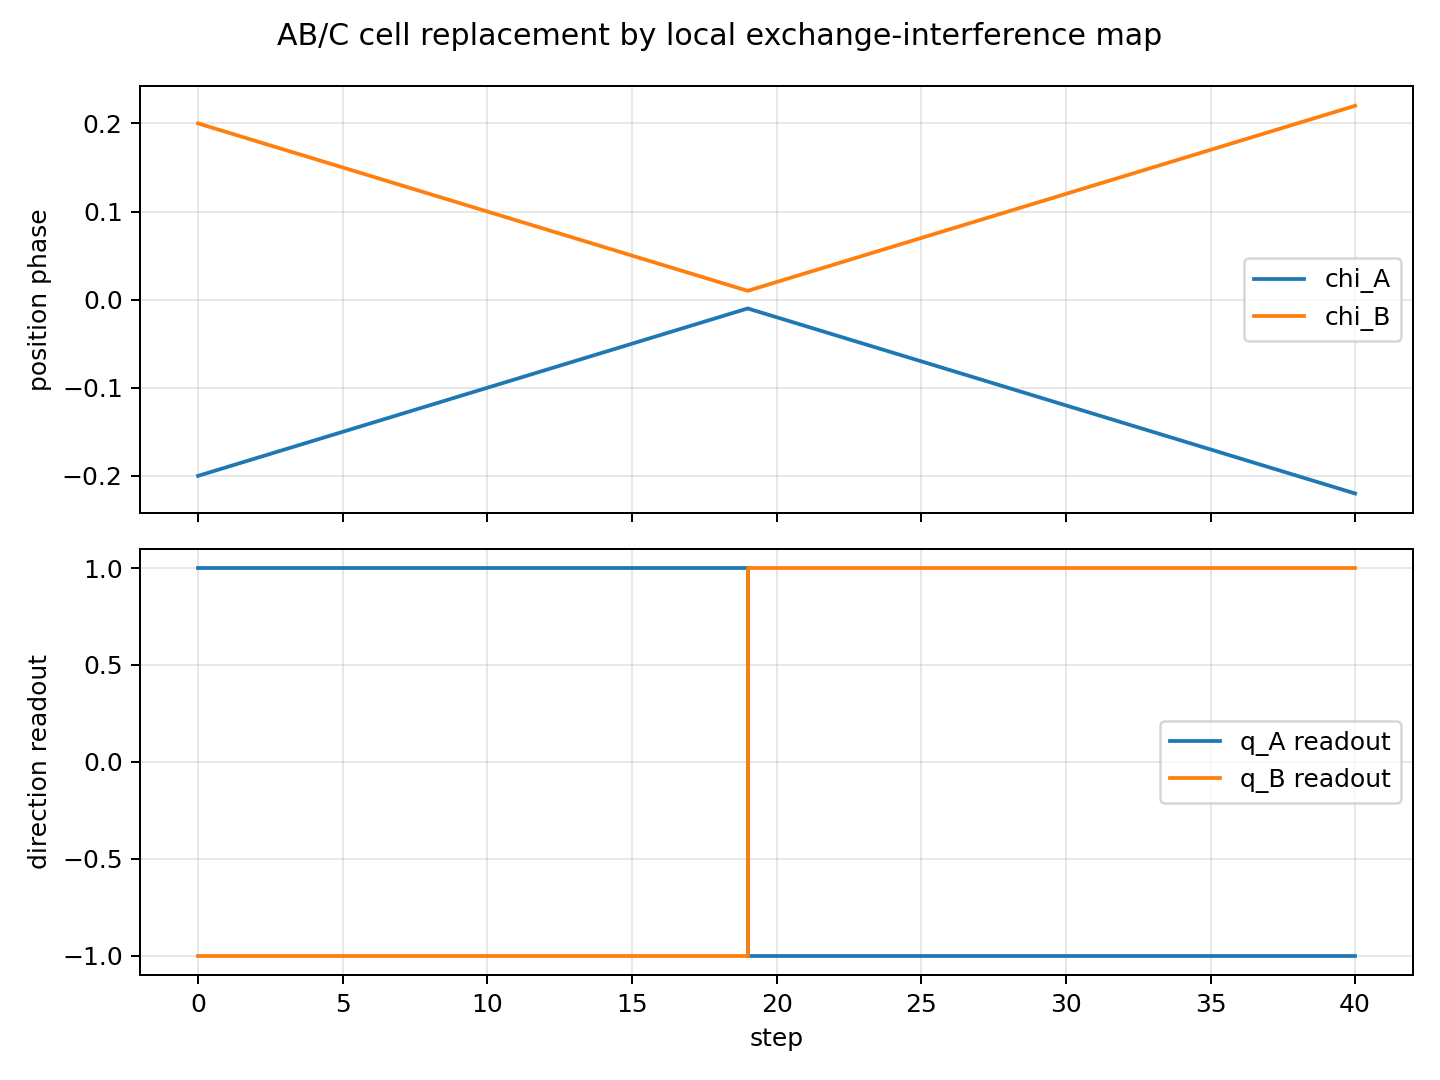
\includegraphics[keepaspectratio,alt={AB/C cell replacement}]{fermionic_interference_reflection_result_v1/fermionic_interference_ab_c_replacement_v1.png}}

\begin{center}\rule{0.5\linewidth}{0.5pt}\end{center}

\subsection{11. Evaluation Quantities}\label{11-evaluation-quantities}

\subsubsection{11.1 Transmission Rate}\label{111-transmission-rate}

\[T
=
\frac{I_{\mathrm{trans}}}
{I_{\mathrm{trans}}+I_{\mathrm{refl}}}.\]

\subsubsection{11.2 Reflection Rate}\label{112-reflection-rate}

\[R
=
\frac{I_{\mathrm{refl}}}
{I_{\mathrm{trans}}+I_{\mathrm{refl}}}.\]

\subsubsection{11.3 Identification-Mode
Readout}\label{113-identification-mode-readout}

\[O_{P,m}^{(j)}
=
\frac{1}{(2\pi)^3}
\iiint
P
C_{\mathrm{read},P}^{(j)}
e^{-im\eta}
\,d\chi d\tau d\eta.\]

\subsubsection{11.4 Expected Phase
Dependence}\label{114-expected-phase-dependence}

For an ideal two-channel interference map,

\[R(\Delta_F)
=
\sin^2\frac{\Delta_F}{2},\]

and

\[T(\Delta_F)
=
\cos^2\frac{\Delta_F}{2}\]

are obtained analytically.

The numerical experiment does not substitute these values directly as
the reflection and transmission rates. It executes free propagation of a
one-sided incident wave packet, local even-odd channel decomposition,
internal phase transfer, and recombination, and then measures
\texttt{R,T} from the final waveform. The phase sweep verifies that the
implemented local exchange-interference map matches the analytic
two-channel map.

\subsubsection{11.5 Closure Residual}\label{115-closure-residual}

\[\mathcal R_{\mathrm{closure}}
=
\left|
\sum_n x_n^2
\right|.\]

\subsubsection{11.6 Reversibility}\label{116-reversibility}

When the reflection-interference process is applied twice,

\[\mathcal U_F^2\approx I\]

is evaluated numerically.

\begin{center}\rule{0.5\linewidth}{0.5pt}\end{center}

\subsection{12. Success Conditions}\label{12-success-conditions}

For the minimal execution in this paper, the construction is judged to
generate the reflection map internally when the following hold.

\begin{enumerate}
\def\labelenumi{\arabic{enumi}.}
\tightlist
\item
  The initial state is a single incident wave packet placed only on the
  left side.
\item
  No external \texttt{q=-q} instruction is used.
\item
  For \texttt{Δ\_F=0},
  \texttt{R\textbackslash{}simeq0,T\textbackslash{}simeq1}.
\item
  For \texttt{Δ\_F=\textbackslash{}pi/2},
  \texttt{R\textbackslash{}simeq\ T\textbackslash{}simeq1/2}.
\item
  For \texttt{Δ\_F=\textbackslash{}pi},
  \texttt{R\textbackslash{}simeq1,T\textbackslash{}simeq0}.
\item
  Over the phase sweep, \texttt{R(Δ\_F)=sin\^{}2(Δ\_F/2)} and
  \texttt{T(Δ\_F)=cos\^{}2(Δ\_F/2)} hold.
\item
  Norm is preserved through propagation and interaction.
\item
  At \texttt{Δ\_F=π}, the complete-overlap diagonal norm decreases to
  numerical-error range.
\item
  Removing the exchange path removes node formation.
\item
  Identification oscillations \texttt{m\_A,m\_B} are preserved by
  readout.
\item
  \texttt{U(π)\^{}2≈I} and \texttt{U(Δ\_F)U(-Δ\_F)≈I} hold.
\item
  The compensated square-closure residual remains below threshold.
\item
  The cell-level direction reversal in the previous AB/C simulation can
  be generated from the local exchange-interference map as
  \texttt{q\_out=q\_in*(T-R)}.
\end{enumerate}

\begin{center}\rule{0.5\linewidth}{0.5pt}\end{center}

\subsection{13. Failure Conditions}\label{13-failure-conditions}

{\def\LTcaptype{none} % do not increment counter
\begin{longtable}[]{@{}ll@{}}
\toprule\noalign{}
Failure condition & Meaning \\
\midrule\noalign{}
\endhead
\bottomrule\noalign{}
\endlastfoot
A node forms but no reflected wave is generated & Transmission
cancellation alone is not enough to generate direction reversal \\
Transmission remains at \texttt{Δ\_F=π} & Amplitude matching or phase
transfer of the exchange path is incomplete \\
Reflection becomes one only after external normalization & Complete
reflection has not been generated by interference alone \\
Identification oscillations are exchanged & Apparent reflection cannot
be distinguished from identity exchange \\
Reflection occurs even without the exchange path & Another numerical
boundary condition may be generating reflection \\
Representative amplitude increases & Recombination normalization is
inappropriate \\
\texttt{R+T} differs from one & The readout definition or closure
condition is insufficient \\
\end{longtable}
}

\begin{center}\rule{0.5\linewidth}{0.5pt}\end{center}

\subsection{14. Discussion}\label{14-discussion}

\subsubsection{14.1 Operation Selection Is Not a
Judgment}\label{141-operation-selection-is-not-a-judgment}

In this construction, a local wave does not recognize itself as a
fermion and then choose an operation.

\[\Delta_F\]

appears directly as the relative phase of the exchange path and
determines the interference result.

Thus the operation selection is not an external judgment. It is a
selection rule for connectable phase channels.

\subsubsection{\texorpdfstring{14.2 No External \texttt{π/2} Adjustment
Is
Required}{14.2 No External π/2 Adjustment Is Required}}\label{142-no-external-ux3c02-adjustment-is-required}

If the complete inversion matrix is written as a two-state rotation, a
\texttt{π/2} angle appears. In this construction, that integrated angle
is not supplied externally.

The direct cause is the complete cancellation of the two exchange paths:

\[1+e^{i\pi}=0.\]

\subsubsection{14.3 Reflection Generation from One-Sided
Incidence}\label{143-reflection-generation-from-one-sided-incidence}

The condition

\[\Psi_F(0)=0\]

alone is not enough to confirm reflection generation. Therefore, this
paper does not begin by placing an odd-function wave. Instead, the
initial state is a single wave packet incident from the left.

The initial right-side probability before interaction is

\begin{Shaded}
\begin{Highlighting}[]
\NormalTok{2.4303500961591473e{-}89,}
\end{Highlighting}
\end{Shaded}

so neither a reflected component nor a mirror component is embedded in
the initial state. After free propagation brings the packet into the
interaction region, the packet is decomposed into even and odd
interference channels, and only the internal core phase \texttt{Δ\_F} is
transferred to the odd channel.

This process gives transmission rate one for \texttt{Δ\_F=0} and
reflection rate one for \texttt{Δ\_F=π}. Reflection is therefore
generated by the local exchange-interference map in the interaction
region, not by a mirror structure in the initial condition.

\subsubsection{14.4 The Implementation Is a Local-Map
Method}\label{144-the-implementation-is-a-local-map-method}

This implementation does not integrate an interaction Hamiltonian
\texttt{H\_int(ρ,Δ\_F)} continuously in time. The computational order
is:

\begin{Shaded}
\begin{Highlighting}[]
\NormalTok{free propagation of a one{-}sided incident packet}
\NormalTok{→ even{-}odd channel decomposition in the interaction window}
\NormalTok{→ transfer of the internal core phase Δ\_F to the odd channel}
\NormalTok{→ recombination}
\NormalTok{→ readout of R,T after free propagation}
\end{Highlighting}
\end{Shaded}

What is confirmed here is that the external \texttt{q=-q} instruction
can be replaced by a local exchange-interference map controlled by the
phase of the internal inverse-phase core.

\begin{center}\rule{0.5\linewidth}{0.5pt}\end{center}

\subsection{15. Conclusion}\label{15-conclusion}

This paper executed a minimal mechanism that internally generates the
direction-reversal map previously introduced as a construction rule
inside a finite-resolution interaction cell, using a fermionic internal
inverse-phase core and two exchange paths.

When the internal phase difference \texttt{Δ\_F} is transferred as the
relative phase between the direct and exchange paths, the waveform at
the complete-overlap point becomes exactly zero under the pure fermionic
condition \texttt{Δ\_F=π}. The execution gave diagonal relative norm
\texttt{7.4987989133092880e-33} at \texttt{Δ\_F=π}, while removing the
exchange path left \texttt{4.9999999999999994e-01}. Thus, node formation
was generated by exchange-path interference.

For one-sided incident local exchange-interference scattering,
\texttt{Δ\_F=0} gave reflection \texttt{1.8261693781071190e-19} and
transmission \texttt{1.0000000000000002}. \texttt{Δ\_F=π/2} gave
reflection and transmission both equal to \texttt{0.5}. \texttt{Δ\_F=π}
gave reflection \texttt{1.0000000000000002} and transmission
\texttt{1.7939211291143336e-19}. Over the phase sweep,
\texttt{R(Δ\_F)=sin\^{}2(Δ\_F/2)} and \texttt{T(Δ\_F)=cos\^{}2(Δ\_F/2)}
held with maximum error \texttt{5.551115123125783e-16}; the maximum norm
error was \texttt{6.661338147750939e-16}.

For reversibility of the local exchange-interference map, the relative
error of \texttt{U(π)\^{}2} was \texttt{4.8214412843789535e-11}, and the
maximum relative error of \texttt{U(Δ\_F)U(-Δ\_F)} was
\texttt{1.4547631339456792e-16}. The maximum compensated square-closure
residual was \texttt{1.2143074258005e-17}.

Finally, in the interaction cell of the previous AB/C complete elastic
collision simulation, the direct \texttt{q} reversal instruction was not
used. The direction readout was generated as \texttt{q\_out=q\_in*(T-R)}
from \texttt{R,T} obtained by the local exchange-interference map. In
this replacement integration test, \texttt{q\_A} changed from
\texttt{1.0} to \texttt{-1.0000000000000002}, \texttt{q\_B} changed from
\texttt{-1.0} to \texttt{1.0000000000000002}, and the identification
oscillations \texttt{m\_A=1} and \texttt{m\_B=2} were preserved from
initial to final readout.

Therefore, without an external conditional branch, artificial
\texttt{q=-q} instruction, mirror-image initial condition, or reflecting
boundary condition, the construction generates the direction-reversal
output corresponding to complete elastic reflection from an internal
inverse-phase core, localized-wave overlap, exchange paths, even-odd
interference channels, local phase transfer, and
identification-oscillation readout.

\begin{center}\rule{0.5\linewidth}{0.5pt}\end{center}

\section{Appendix A. Executed Program and
Outputs}\label{appendix-a-executed-program-and-outputs}

The program used in this execution is:

\begin{Shaded}
\begin{Highlighting}[]
\NormalTok{run\_fermionic\_interference\_reflection\_v1.py}
\end{Highlighting}
\end{Shaded}

The output directory is:

\begin{Shaded}
\begin{Highlighting}[]
\NormalTok{fermionic\_interference\_reflection\_result\_v1/}
\end{Highlighting}
\end{Shaded}

The main outputs are:

{\def\LTcaptype{none} % do not increment counter
\begin{longtable}[]{@{}ll@{}}
\toprule\noalign{}
Type & File \\
\midrule\noalign{}
\endhead
\bottomrule\noalign{}
\endlastfoot
Execution report &
\href{fermionic_interference_reflection_result_v1/fermionic_interference_reflection_report_v1.md}{fermionic\_interference\_reflection\_report\_v1.md} \\
Result JSON &
\href{fermionic_interference_reflection_result_v1/fermionic_interference_reflection_result_v1.json}{fermionic\_interference\_reflection\_result\_v1.json} \\
Phase-sweep CSV &
\href{fermionic_interference_reflection_result_v1/fermionic_interference_phase_sweep_v1.csv}{fermionic\_interference\_phase\_sweep\_v1.csv} \\
Relative-dynamics CSV &
\href{fermionic_interference_reflection_result_v1/fermionic_interference_relative_dynamics_v1.csv}{fermionic\_interference\_relative\_dynamics\_v1.csv} \\
One-sided scattering CSV &
\href{fermionic_interference_reflection_result_v1/fermionic_interference_single_sided_scattering_v1.csv}{fermionic\_interference\_single\_sided\_scattering\_v1.csv} \\
Reversibility CSV &
\href{fermionic_interference_reflection_result_v1/fermionic_interference_reversibility_sweep_v1.csv}{fermionic\_interference\_reversibility\_sweep\_v1.csv} \\
AB/C replacement CSV &
\href{fermionic_interference_reflection_result_v1/fermionic_interference_ab_c_replacement_timeline_v1.csv}{fermionic\_interference\_ab\_c\_replacement\_timeline\_v1.csv} \\
Exchange-interference node figure &
\href{fermionic_interference_reflection_result_v1/fermionic_interference_phase_sweep_v1.png}{fermionic\_interference\_phase\_sweep\_v1.png} \\
Relative-dynamics figure &
\href{fermionic_interference_reflection_result_v1/fermionic_interference_relative_dynamics_v1.png}{fermionic\_interference\_relative\_dynamics\_v1.png} \\
One-sided scattering figure &
\href{fermionic_interference_reflection_result_v1/fermionic_interference_single_sided_scattering_v1.png}{fermionic\_interference\_single\_sided\_scattering\_v1.png} \\
AB/C replacement figure &
\href{fermionic_interference_reflection_result_v1/fermionic_interference_ab_c_replacement_v1.png}{fermionic\_interference\_ab\_c\_replacement\_v1.png} \\
\end{longtable}
}

The execution command is:

\begin{Shaded}
\begin{Highlighting}[]
\NormalTok{python3 run\_fermionic\_interference\_reflection\_v1.py}
\end{Highlighting}
\end{Shaded}

This implementation does not use external direction-reversal
substitution. The verdict in the result JSON is:

\begin{Shaded}
\begin{Highlighting}[]
\NormalTok{external\_q\_flip\_used: false}
\NormalTok{single\_sided\_initial\_packet: true}
\NormalTok{dynamic\_transmission\_at\_zero: true}
\NormalTok{dynamic\_half\_phase\_split: true}
\NormalTok{dynamic\_reflection\_at\_pi: true}
\NormalTok{dynamic\_phase\_sweep\_matches\_expected: true}
\NormalTok{dynamic\_norm\_preserved: true}
\NormalTok{static\_node\_at\_pi: true}
\NormalTok{phase\_sweep\_matches\_expected: true}
\NormalTok{exchange\_path\_required: true}
\NormalTok{label\_mode\_preserved\_A: true}
\NormalTok{label\_mode\_preserved\_B: true}
\NormalTok{pi\_twice\_reversible: true}
\NormalTok{inverse\_sweep\_reversible: true}
\NormalTok{compensated\_square\_closure\_preserved: true}
\NormalTok{ab\_c\_replacement\_valid: true}
\NormalTok{mechanism\_valid\_minimal: true}
\end{Highlighting}
\end{Shaded}

\begin{center}\rule{0.5\linewidth}{0.5pt}\end{center}

\section{Appendix B. Treatment of the Earlier
Draft}\label{appendix-b-treatment-of-the-earlier-draft}

The earlier program draft generated by ChatGPT is not used for the
verdict in this paper. Its \texttt{exchange\_coordinates()} operation
was a reversal of a one-particle waveform and did not explicitly
construct the two-particle direct path \texttt{P\_A(1)P\_B(2)} and
exchange path \texttt{P\_A(2)P\_B(1)}.

The present execution replaces it with an implementation that satisfies
the following:

\begin{enumerate}
\def\labelenumi{\arabic{enumi}.}
\tightlist
\item
  The direct and exchange paths are explicitly compared on the
  complete-overlap diagonal.
\item
  The diagonal norm is measured to vanish at \texttt{Delta\_F=pi}.
\item
  Removing the exchange path is measured to remove node formation.
\item
  A one-sided incident packet is propagated and \texttt{R,T} are
  measured for \texttt{Δ\_F=0,\textbackslash{}pi/2,\textbackslash{}pi}
  and over the full phase sweep.
\item
  The single free packet and odd-node half-line readout are retained as
  auxiliary checks.
\item
  The \texttt{η} identification oscillation is separated from the
  reflection-generating channel and checked as a preserved readout
  channel.
\item
  No external direction-reversal instruction \texttt{q=-q} is used.
\end{enumerate}

With this replacement, the earlier draft remains only as a design note,
and the execution basis of the paper is unified around the executed
program and outputs listed in Appendix A.

\end{document}
